\documentclass[10pt,twocolumn]{article}

\usepackage[margin=0.9in,columnsep=0.25in]{geometry}
\usepackage{graphicx}
\usepackage{booktabs}
\usepackage{amsmath,amssymb}
\usepackage{microtype}
\usepackage{xcolor}
\usepackage[hidelinks]{hyperref}
\usepackage{caption}
\captionsetup{font=small,labelfont=bf}
\usepackage{titlesec}
\titlespacing*{\section}{0pt}{9pt}{4pt}
\titlespacing*{\subsection}{0pt}{7pt}{3pt}

\newcommand{\sys}{\textsc{hytorch}}
\newcommand{\hyphae}{\textsc{Hyphae}}
\definecolor{darkred}{RGB}{176,58,46}
\newcommand{\finding}[1]{\textcolor{darkred}{\textbf{#1}}}

\title{\textbf{The Missing Medium:\\ A Transactional Residual Stream for Transformer Training}}
\author{
  Hyphae Research Foundation\\[2pt]
  \small Version 1.1 --- 5 September 2026 (v1.0: 4 September; reframed after four external reviews, see \texttt{paper/notes/REVIEWS-2026-09.md}).\\
  \small Preprint DOI: \href{https://doi.org/10.5281/zenodo.22059493}{10.5281/zenodo.22059493}. Code and evidence: \url{https://github.com/Hyphae-Research-Foundation/hytorch} (release v1.1).\\
  \small Code: Apache-2.0. This document, its figures and the results it cites: CC BY-SA 4.0.\\
  \small Every number traces to a file in \texttt{results/} or a record key in a \hyphae{} ledger (\S\ref{sec:evidence}).
}
\date{}

\begin{document}
\maketitle

\begin{abstract}
Modern training treats the transformer residual stream as an anonymous
accumulator: any kernel may execute $h \mathrel{+}= \delta$, and no record of
the write survives the step. Training observes the \emph{consequences} of
internal writes --- loss curves, evaluations, activation probes --- never the
writes themselves. We introduce \sys{}, a training loop in which the residual
stream is a \emph{typed, transactional channel}: blocks propose, a pinned
policy admits, and every candidate write leaves exactly one 16-byte record
--- \textsc{commit}, \textsc{overflow} (lost a slot contention) or
\textsc{abort} (rule rejection) --- so that what the model \emph{attempted}
to write, and why it was refused, is data. Every optimizer step is gated by a
durable receipt from an embedded transactional store (\hyphae{}); a CPU-only
verifier replays audited microbatches bit-for-bit against a pinned software
reference; the same reference binary admits NVIDIA (sm\_89/sm\_90), AMD
(gfx950) and, through a two-phase policy, AWS Trainium2 kernels on 200{,}000
adversarial cases with bit-identical verdicts and residuals. Fault injection
over real training spills is detected 36/36 with the correct class.

The instrument produced two results. Our preregistered protocol reversed our
own headline: a single-LR $-44.9\%$ perplexity win, replicated across
vendors, became a $2.9\times$ loss to the properly tuned dense twin under the
preregistered LR sweep, and we publish the reversal. And at nanochat-d20 scale
the ledger recorded a \emph{silent channel collapse}: commit rate
$0.066\%\!\to\!0$ by step 200, the write codebook frozen bit-exactly, while
validation loss improved on schedule through the architecture's declared
bypass paths. Neither loss, evaluation nor activation probes distinguish an
expensive pathway from a dead one; the write records do, mechanically, during
training. We are explicit about what this is and is not. \sys{} is an
instrumentation and verification framework, not an efficient training
architecture: the channel configuration we tested (at most 160 scalar degrees
of freedom per token per layer) does not carry a language model --- the
cataloged d20 model is at chance on knowledge tasks --- and costs
$12$--$29\times$ the twin's wall clock; its headline capacity number comes
from a run whose STE gradient we later found to be mis-scaled, and the
corrected rerun does not yet exist. What the evidence supports is narrower and,
we argue, more useful: a training process whose state transitions through the
typed channel are witnessed, receipted and replayable.
\end{abstract}

\section{Introduction}
\label{sec:intro}

A transformer's residual stream is its only inter-layer medium: every head
and every MLP communicates by adding into it. Yet in every production
training stack this medium is an \emph{anonymous accumulator}. Writes carry
no identity, no admission decision, no durable trace; the optimizer steps
whether or not anything about those writes was ever inspected. All
observability is reconstructed after the fact from the outside (loss curves,
evals, activation probes) --- none of it witnesses the \emph{acts}.

\sys{} makes the acts the unit of record. The residual stream becomes a
typed, transactional channel: blocks \emph{propose} deltas; a pinned policy
object packs proposals against a learned write codebook, allocates winners
per slot, and \emph{applies} only committed bindings. Every candidate ---
including every rejected one --- becomes a 16-byte record in a durable
ledger, and \texttt{optimizer.step()} is legal only after the step's records
have a commit receipt. Figure~\ref{fig:arch} shows the seam. To our
knowledge, prior systems do not combine residual-write journaling, durable
per-step receipts and bit-exact replay at this granularity
(\S\ref{sec:related}); we do not claim more priority than that.

Three words recur below and are used in their narrow senses.
\emph{Observability}: we know which writes occurred and which were refused.
\emph{Auditability}: we can show they occurred and were not altered
(tamper-evident, not unforgeable). \emph{Replayability}: a CPU can reproduce
them bit for bit. We make no claim of \emph{interpretability} (what a write
means) beyond one small probe, and no claim of \emph{causality} (that a write
causes a behaviour) beyond one journalized intervention; both are marked
where they appear.

The contributions are:
\begin{itemize}\itemsep2pt
  \item \textbf{C1 (transactional residual stream):} a training loop where
  residual writes are typed transactions with verdicts, the negative space
  (\textsc{overflow}, \textsc{abort}) is recorded as data, receipts gate the
  optimizer, and a CPU replays audited steps bit-exactly
  (\S\ref{sec:design}--\ref{sec:seam}).
  \item \textbf{C2 (deterministic cross-silicon semantics):} one reference
  binary admits NVIDIA and AMD kernels to \emph{bit-identical} verdicts and
  residuals on 200k adversarial cases; the port to AWS Trainium2 moved the
  verification boundary without weakening it, and the channel trains there
  under DDP with every step receipted (\S\ref{sec:gates},
  \S\ref{sec:twophase}).
  \item \textbf{C3 (mechanical observability, including of ourselves):}
  36/36 injected faults caught with the correct class, and a preregistered
  evaluation whose sweep reversed our own replicated headline
  (\S\ref{sec:prereg}).
  \item \textbf{C4 (the finding):} silent channel collapse --- a
  load-bearing internal pathway can die completely while training telemetry
  reads healthy, because the host architecture carries the trunk through
  declared bypass paths. Write-level records distinguish this from a merely
  expensive pathway during training; observational activation evidence alone
  cannot (\S\ref{sec:collapse}).
  \item \textbf{C5 (what it costs):} with the channel verifiably alive at
  d20, the configuration tested does not carry a language model and costs
  $12\times$ (exact kernels) to $29\times$ (two-phase) the twin's wall clock;
  we report this as the measured price of the instrument as configured, with
  the caveats it carries (\S\ref{sec:price}).
\end{itemize}
In one line: make the writes observable (C1), make them deterministic (C2),
make the experiment adversarial to our own claims (C3), show what becomes
visible once the writes are witnessed (C4), and say what it costs (C5).

\begin{figure*}[t]
  \centering
  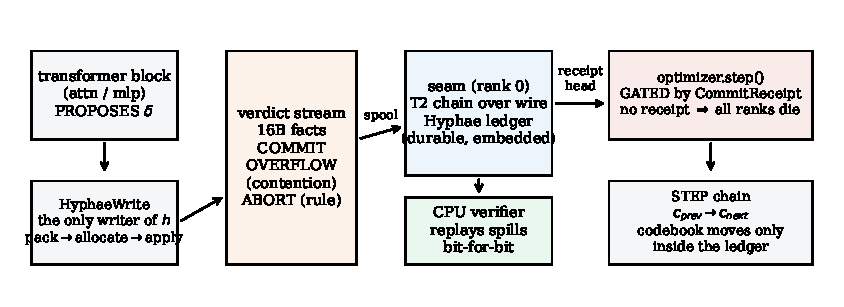
\includegraphics[width=\textwidth]{figs/fig5_architecture.pdf}
  \caption{The \sys{} seam. Blocks propose; \texttt{HyphaeWrite} is the only
  writer of the residual. The verdict stream (16-byte facts: commits,
  contentions, rule rejections) is spooled to a rank-0 seam that chains it
  (T2) into an embedded \hyphae{} ledger. The optimizer is gated by the
  commit receipt; the codebook may move only inside the ledger
  ($c_{\text{prev}} \to c_{\text{next}}$ chain). A CPU verifier replays
  audited microbatches bit-for-bit.}
  \label{fig:arch}
\end{figure*}

\section{Design: five laws}
\label{sec:design}

\textbf{Law 0 (single writer, declared exceptions).} Within a block, the
catalog write is the only mutation of $h$: attention and MLP outputs are
\emph{proposals} $\delta$, not writes. Host architectures may carry
residual mutations \emph{outside} the block (nanochat's per-layer
$x \leftarrow \lambda_i x + \mu_i x_0$ scalars and smear/backout gates).
These are not silenced and not pretended away: they are declared in the
manifest and journalized every step as a \textsc{bypass} fact (the scalar
values), so an auditor sees exactly which writes went through the typed
channel and which did not. \S\ref{sec:collapse} shows why this matters.

\textbf{Law 1 (typed writes).} A write is a binding $(pos, slot, feature,
mag)$: magnitude $\times$ unit-normalized codebook row, applied to one slot
of one token. $k$ candidates per token; one winner per slot.

\textbf{Law 2 (verdicts are facts).} Every candidate leaves exactly one
fact: \textsc{commit}, \textsc{overflow} (lost a slot collision), or
\textsc{abort} (nonfinite, magnitude cap, or policy denial). The negative
space is journalized, not dropped: \#C + \#O + \#A $= k$, always.

\textbf{Law 3 (receipts gate the step).} All ranks spool their frames; rank
0 waits for the ledger's commit receipt and broadcasts its head; a missing
receipt kills all ranks. There are no ledger-less steps --- we verified this
the hard way (\S\ref{sec:collapse}, incidents).

\textbf{Law 4 (replayability).} The bf16 bit-contract (promote, fp32
sequential no-FMA reductions, RNE downcast, canonical NaN) is pinned in a
reference object whose SHA-256 is cited by every run. A CPU replay of any
audited microbatch reproduces residuals bit-for-bit.

\section{The pinned reference and per-silicon gates}
\label{sec:gates}

The policy (pack $\to$ allocate $\to$ apply) exists once, as a Rust
reference compiled to \texttt{libapply\_ref.so}; CUDA (sm\_89/sm\_90) and
HIP (gfx950) kernels are \emph{admitted} per silicon by a differential
harness: 200{,}000 adversarial cases in total, drawn round-robin from seven
generator families (NaN/Inf floods, denormals, cap boundaries, tie storms,
\ldots) under a fixed seed --- i.e.\ $\sim$28k per family, reproducible
rather than fresh per run --- must produce byte-identical verdict records
and residuals. A single canonicalization rule (NaN $\to$ +qNaN before ordering)
was required to make x86 and device NaN semantics agree --- found by the
gate, not by inspection. The kernels use a packed $(key, feature)$
comparator so parallel argmax equals the reference's sequential tiebreak
exactly.

Fault injection (Fig.~\ref{fig:inject}): 36 mutations across six classes
(bit-flipped magnitudes, dropped/injected commits, reordered application,
wrong codebook row, truncated wire) against real training spills; 36/36
detected, each with the correct failure class (head mismatch, apply error,
or chain break).

\begin{figure}[htbp]
  \centering
  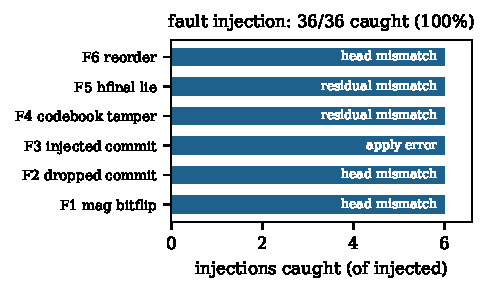
\includegraphics[width=0.92\columnwidth]{figs/fig4_inject.pdf}
  \caption{Fault injection over real training spills: 36/36 caught, correct
  class each. \texttt{results/inject/inject-summary.json}.}
  \label{fig:inject}
\end{figure}

\section{Authority $\neq$ durability: the seam}
\label{sec:seam}

The trainer holds \emph{authority} (it computes); the ledger holds
\emph{durability} (it remembers). The seam is a rank-0 process consuming
per-layer wire frames, walking a hash chain (T2) over every fact, and
committing \{layer records, receipt, step chain\} transactionally into
\hyphae{}, an embedded store. Two costs must be kept apart. The
\emph{seam} overhead --- spooling, chaining, committing --- is 9.5\% of wall
clock at 20k steps on one GPU and $\sim$5\% amortized at
nanochat-d20$\times$8 ranks (335M facts/step; the T2 chain and counts are
durable for \emph{every} step, raw wire sampled at a declared cadence). The
\emph{channel} cost --- running pack/allocate/apply for 40 write units over
a 32{,}768-feature codebook in the forward and its mirror in the backward
--- is far larger: at d20 on 8$\times$MI355X the catalog arm ran at
\textbf{7.42\,s/step vs.\ 0.62\,s/step} for the dense twin (12$\times$
wall clock; \texttt{results/models/d20-3.4/NOTES.md}), with the exact
device kernels executing the full $N_f$ scan. Two-phase selection
(\S\ref{sec:twophase}) removes the exact scan from the device but pays a
host round trip per write unit instead: 29$\times$ at d10 on Trainium2.
Readers should take 12$\times$ (exact kernels) to 29$\times$ (two-phase),
not 9.5\%, as the current end-to-end price of the typed channel.

Records scale: the d20 runs produce $3.4\times10^{8}$ verdict records per
optimizer step ($1.7\times10^{12}$ per full run). What is durable for
\emph{every} step is the T2 chain head, the per-layer counts and the receipt;
the raw 16-byte records themselves ($\sim$55\,TB per run at full cadence) are
retained at a declared cadence (every 100 steps). ``Receipted on 100\% of
steps'' therefore means every step's writes are chained and countable, not
that the full transcript is stored.

\emph{What a receipt guarantees.} The receipt is the head of an unkeyed
SHA-256 chain over every fact of the step, stored transactionally. It is
\emph{tamper-evident}: any post-hoc modification, drop, reorder or
injection of a fact is detected (\S\ref{sec:gates}, 36/36). It is not
\emph{unforgeable}: an adversary who controls the seam process could
fabricate an internally consistent chain from scratch. Unforgeability
requires keying or external anchoring of heads (a straightforward
extension we have not built); every claim in this paper is an integrity
claim, not a non-repudiation claim.

\section{Preregistration catches our own headline}
\label{sec:prereg}

Phase 1's preregistered gate (PPL gap $\le 10\%$ vs a \emph{topology-matched}
dense twin --- same depth, width, data and schedule; the catalog arm carries
$\sim$3.5\% more theoretical FLOPs and an order of magnitude more wall
clock, so ``FLOPs-matched'' would overstate the parity --- wikitext-103) \textbf{failed} honestly ($+11.17\%$); a spec amendment
(removing a ReZero-style gate that stabilized the dense twin) produced a
\textbf{pass}: catalog $167.8$ vs twin $304.7$ ($-44.9\%$), replicated on
AMD ($-43.2\%$), $930/930$ audited microbatches green across three seeds.

The preregistration also demanded an LR sweep before any claim.
Figure~\ref{fig:lrsweep} shows what it found: the dense twin at its own best
LR beats the catalog $2.9\times$; the $-44.9\%$ was an artifact of comparing
both arms at the one LR where the twin destabilizes. What survives is real
but different: the catalog is $6\times$ more LR-robust and $7\times$ more
seed-stable (Fig.~\ref{fig:seeds}) --- a stabilizer, not a free win. We
publish the reversal; C1/C2 never depended on winning perplexity.

\begin{figure}[htbp]
  \centering
  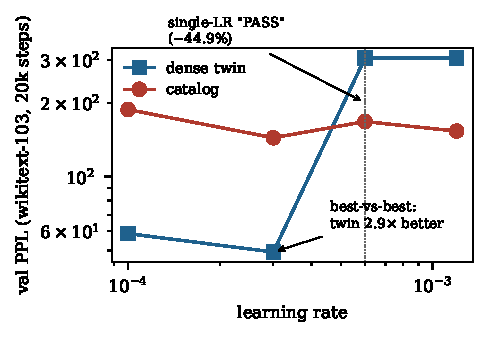
\includegraphics[width=0.95\columnwidth]{figs/fig2_lrsweep.pdf}
  \caption{The preregistered LR sweep reverses the single-LR headline.
  \texttt{results/train/NVIDIA-H200/lrsweep-*/NOTES.md}.}
  \label{fig:lrsweep}
\end{figure}

\begin{figure}[htbp]
  \centering
  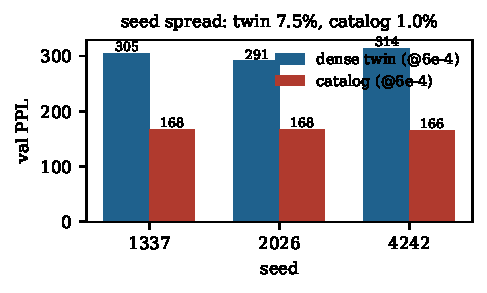
\includegraphics[width=0.95\columnwidth]{figs/fig3_seeds.pdf}
  \caption{What survived the sweep: the catalog's seed variance is
  $7\times$ smaller than the dense twin's (at the twin-unstable LR).}
  \label{fig:seeds}
\end{figure}

\section{The finding: silent channel collapse}
\label{sec:collapse}

Scaling to nanochat-d20 (1.9B-token compute-optimal horizon, 8$\times$MI355X,
$d_{\text{model}}{=}1280$, 40 write units, $k{=}8$, magnitude cap 64), the
ledger recorded the following (Fig.~\ref{fig:collapse}): at step 100 the
commit rate was $0.066\%$ with surviving magnitudes pinned to the cap
(p50 $=58$ of 64); by step 200 it was \emph{exactly zero} and stayed zero.
Proposals grew to $10^5$--$3.7\times10^{6}$ (up to $58{,}000\times$ the
cap). With zero commits the straight-through gradient path dies; the
codebook's STEP chain shows $c_{\text{prev}} = c_{\text{next}}$ --- frozen
bit-exactly. \emph{Meanwhile validation bits-per-byte improved on
schedule} (3.17 $\to$ 1.32 by step 750): nanochat's bypass parameters
($x_0$/residual scalars, value embeddings) let the model learn
\emph{around} its dead channel.

\begin{figure*}[t]
  \centering
  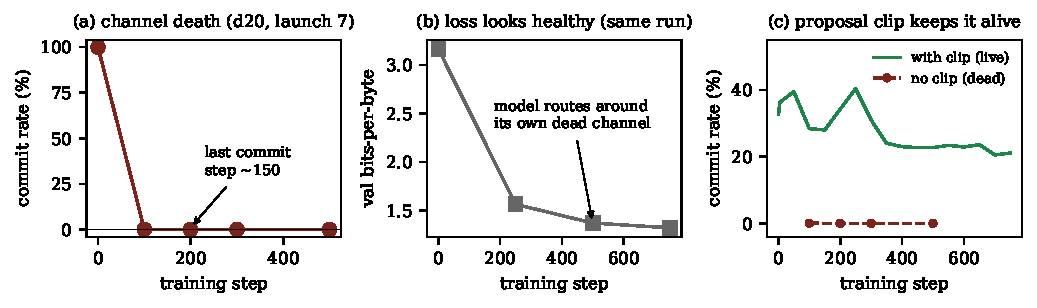
\includegraphics[width=\textwidth]{figs/fig1_collapse.pdf}
  \caption{Silent channel collapse at d20. (a) Commit rate measured from
  retained wire (335M facts/step): dead by step 150--200. (b) The same
  run's validation loss improves normally --- the model routes around the
  dead channel. (c) With the proposal clip the channel stays alive at the
  same scale. \texttt{results/nanochat/PHASE5-CHANNEL-COLLAPSE.md}.}
  \label{fig:collapse}
\end{figure*}

Mechanism: raw attention/MLP outputs at $d{=}1280$ already sit near the cap
at init; LR warmup pushes the distribution through it; overflow/abort
$\Rightarrow$ no gradient $\Rightarrow$ no correction --- a one-way feedback
loop into permanent death. The fix is a per-slot proposal norm clip at
cap$/2$ before the pack (direction preserved); with it the channel holds a
20--40\% commit rate at the same scale (Fig.~\ref{fig:collapse}c), with the
collapse telemetry now printed in the trainer log every 50 steps.

This is not a new phenomenon: it is codebook collapse (VQ-VAE) and router
collapse (mixture-of-experts) wearing a training-time mask, and a smaller
instance had already occurred in phase 1 at cap 8 (``\textsc{commit}=2,
\textsc{overflow}=118{,}986, loss kept dropping''), then ``fixed'' by
raising the cap the toy inherited. What \emph{is} new is that the ledger
exposes it mechanically and that our phase-1 manifests had preregistered a
codebook-usage-entropy kill threshold that no code implemented --- a gap
between promise and guard that this incident closed: the threshold (8 bits
usage entropy, 2\% commit rate, sustained 50 steps) now executes inside the
seam and kills all ranks.

Three consequences follow. First, our earlier d20 ``capacity cost''
measurements were measurements of a bypass model, and we reinterpret them as
such. Second, the C1/C3 thesis is demonstrated on this stack: ``expensive
channel'' and ``dead channel with bypass'' are indistinguishable from
outside and mechanically distinct in the records. Third, a consequence for
mechanistic interpretability, stated at the strength the evidence supports:
a claim of the form ``this observed mechanism explains the behaviour''
cannot be established from observational activation evidence alone, because
the model may be using another path --- here it was. Interventional methods
(activation patching, ablation, causal tracing) can establish it; a write
ledger establishes it for the writes it witnesses, which in \sys{} are those
of the typed channel and the declared bypass scalars, not every path. Our
sibling project independently adopted a grad-norm ``dead channel guard''
after this incident; it catches the total-freeze case but not partial
bypass --- only per-write verdicts see that.

Two things this finding is not. It is not a discovery of collapse: VQ
codebooks and MoE routers collapse, and the literature has remedies
(\S\ref{sec:related}). What is new is the ability to tell, during training
and from write-level evidence, a dead internal pathway from an expensive
functioning one. Nor is it yet a law of the residual stream. The host is
nanochat, whose per-layer $x \leftarrow \lambda_i x + \mu_i x_0$ scalars are
a trunk sufficient to carry the loss; in a pre-LN architecture without such
scalars a dead channel might break the loss instead of hiding. How much of
the silence is Law 0's declared bypass and how much is the VQ bottleneck is
open; the guard is the same in either case. Phrases such as ``the model
learned to route around its channel'' are our interpretation of the records
(commits at zero, bypass scalars journalized and moving, loss falling); the
records establish the correlation, not the mechanism.

\section{What it costs}
\label{sec:price}

\paragraph{A caveat before the number.} The d20 pretraining reported here ran
with a gradient bug we found later, while chasing an SFT-stage NaN: the
proposal clip was applied to the \emph{detached} input inside the write
Function, so the STE mirror returned gradients for the clipped proposal that
flowed into the unclipped block output, over-weighted by the clip ratio (up
to $400\times$ at d20) and compounding to \texttt{inf} within 13 layers on
the fine-tuning distribution. The fix (clip in-graph, so the policy judges
exactly what autograd sees) is in the code and in the Trainium2 run of
\S\ref{sec:twophase}; the d20 rerun with the corrected mirror does not yet
exist. The records and receipts are unaffected --- the ledger stores what was
written, not what gradient was returned --- but Table~\ref{tab:price} is the
result of \emph{that} run and must be read as such: because this run
predates the corrected STE mirror, CORE 0.015 should not be interpreted as a
clean estimate of the configuration's capacity ceiling --- it is the observed
result of the current live-channel run, confounded by the now-identified
bug, and the rerun is the definitive measurement. We keep it because it is
the only full-horizon measurement with a verifiably live channel that we
have, and because the qualitative conclusion below does not rest on it alone.

With the clip and the executable guard in place, the d20 catalog arm trained
for the full 4{,}980-step compute-optimal horizon on 8$\times$MI355X with
the channel alive on every step (commit 19--40\%, abort 0.0\%, codebook
usage entropy $>8$ bits, receipts on every step, zero ledger-less steps;
20.8\,h wall, no preemption). The dense twin trained the same steps on the
same data and silicon in 1.7\,h. The twin's per-step validation log was
lost with its droplet --- a custody script that tore down before verifying
its upload; it now hashes every artifact and exits nonzero on any gap --- so
CORE on both final checkpoints is the comparison.

\begin{table}[h]
\footnotesize\centering
\begin{tabular}{@{}lrr@{}}
\toprule
 & catalog (live) & dense twin \\
\midrule
final train loss & 4.08 & 2.39 \\
val bits-per-byte (final / min) & 1.245 / 1.227 & --- \\
\textbf{CORE} (22 tasks, centered) & \textbf{0.015} & \textbf{0.236} \\
seconds / step & 15.0 & 1.2 \\
\bottomrule
\end{tabular}
\caption{Phase 5, nanochat d20, 4{,}980 steps; catalog run with the
mis-scaled STE gradient (see text). CORE from nanochat's \texttt{base\_eval}
on both final checkpoints. \texttt{results/models/d20-p5/}.}
\label{tab:price}
\end{table}

\begin{figure*}[t]
  \centering
  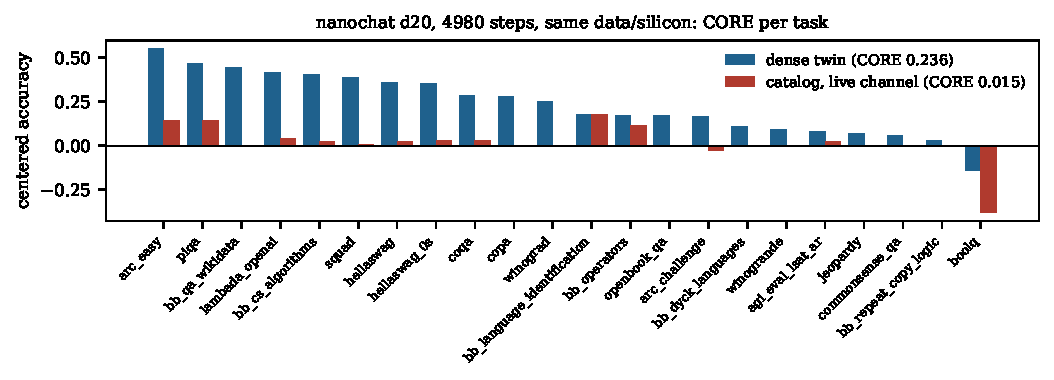
\includegraphics[width=\textwidth]{figs/fig7_core.pdf}
  \caption{CORE per task. The live catalog model is at chance on every
  knowledge- or reasoning-bearing task (Jeopardy $0.0005$ vs $0.070$,
  Wikidata QA $0.0008$ vs $0.447$, LAMBADA $0.039$ vs $0.418$, SQuAD $0.009$
  vs $0.389$) and matches the twin only on format-like tasks. Run with the
  mis-scaled STE gradient (\S\ref{sec:price}).}
  \label{fig:core}
\end{figure*}

The configuration tested is too narrow, and that conclusion does not
rest on the contaminated CORE alone. At $k{=}8$ commits per token per write
unit, each a bf16 magnitude along one of 32{,}768 unit vectors of dimension
20 occupying one of 64 slots, the channel carries at most 160 scalar degrees
of freedom per token per layer against the twin's 1{,}280 free dimensions;
the training loss plateaued near 4.4 from step 1{,}000 to 3{,}000 while the
twin kept descending; and the bypass scalars (Law 0) carried the trunk. We
do not conclude that a transactional residual stream cannot carry a language
model --- we have one policy point, chosen to be verifiable rather than
sufficient. The controls a capacity claim needs are missing and named: a
dense bottleneck of comparable degrees of freedom, a sweep over $k$
($8\to16\to32\to64$) or over fewer, wider slots, and the catalog as an
audited side-channel rather than the sole writer. Each is a rerun we have not
funded.

Table~\ref{tab:cost} separates the three costs the wall-clock numbers mix:
model compute, the channel's own selection work, and verification.

\begin{table*}[t]
\footnotesize\centering
\begin{tabular}{@{}lll@{}}
\toprule
 & dense twin & catalog \\
\midrule
model FLOPs (theoretical) & $1\times$ & $\approx1.035\times$ \\
pack / allocate / apply & --- & full $N_f$ scan on device (kernels) \\
 & & or top-$M$ device + exact host dispose (policy 7) \\
seam: spool, T2 chain, commit & --- & 9.5\% wall (1 GPU, 20k steps); $\sim$5\% at d20$\times$8 \\
host round trips per step & 0 & 0 (kernels); 40 (policy 7, 20 units $\times$ 2 microbatches) \\
records per step (d20) & --- & $3.4\times10^{8}$; chain + counts durable, raw sampled 1/100 \\
wall, d20 4{,}980 steps, 8$\times$MI355X & 1.7\,h (1.2\,s/step) & 20.8\,h (15.0\,s/step), $12\times$ \\
throughput, d10 400 steps, trn2.3xlarge & 84.5k tok/s & 2.8k tok/s, $29\times$ \\
device memory & not measured & not measured (DBS=16 OOM at d10, DBS=4 fits) \\
\bottomrule
\end{tabular}
\caption{Where the cost is. The channel's selection work (exact kernels) or
its host round trips (policy 7) dominate; the ledger itself is under 10\%.
Sources: \texttt{results/models/d20-p5/}, \texttt{results/trn2-d10/},
\texttt{results/train/}.}
\label{tab:cost}
\end{table*}

\section{Any-silicon records: two-phase selection}
\label{sec:twophase}

Porting to AWS Trainium2 forced a question our CUDA/HIP kernels had begged:
what happens on silicon where the pinned sequential math cannot run at
useful throughput? Policy 7 (\emph{two-phase top-$k$},
Fig.~\ref{fig:twophase}) answers: the \emph{device proposes} --- bf16
matmul scores, top-$M$ candidate features per token, XLA-compiled, never
trusted --- and the \emph{reference disposes}: it recomputes the $M$
candidate scores with the pinned math (a $1000\times$ smaller problem) and
runs the unchanged policy-6 verdict machinery. Facts remain bit-exactly
verifiable and replayable (T1/T2/apply unchanged); what is \emph{declared}
rather than verified is proposal completeness, which becomes a measured
miss-rate with a preregistered threshold. \textbf{Measured on Trainium2}
(trn2.3xlarge, torch\_xla/Neuron): device-proposal miss-rate $0.000\%$ across
four adversarial batteries, every committed magnitude equal to the exact
host recompute, and residuals equal to the reference replay bit-for-bit ---
the latter only after moving the apply to the host as well, because the
Neuron compiler does not honor the bf16 contract (1--4\,ulp drift on every
touched leaf). ``Reference disposes'' now covers selection \emph{and} apply.
A gated bridge test proves policy 7 with $M{=}N_f$ is byte-identical to
policy 6.

\textbf{Policy 7 trains on Trainium2 at d10 (60M), catalog vs.\ twin.}
DDP over the four logical NeuronCores of a trn2.3xlarge, 400 steps at
TBS 32k, the same seam, receipts and executable guard as on NVIDIA/AMD:
the cataloged model reaches loss 4.667 against the dense twin's 3.414 (same
tree, same seed and data order; twin/catalog at step 100: 5.21/5.36, step
200: 4.64/5.18), with 400/400 receipts, a continuous STEP chain, $5.2\times
10^{6}$ facts per step and a channel that stays alive throughout --- commit
13--14\% of the $k{=}8$ candidates per token, 86\% \textsc{overflow}, 0\%
\textsc{abort}, codebook usage entropy rising from 5.0 bits at step 50 to
9.0 bits at step 350 (3,062 distinct features). Throughput is the honest
number: 2.8k tok/s against the twin's 84.5k, a $29\times$ cost, all of it in
the per-write-unit host round trip (20 units $\times$ 2 microbatches per
step) rather than the device proposer; a two-pass forward (propose every
unit, dispose once, apply once) is the lever and is future work.

The guard fired twice before that run completed, and both firings are part
of the result. The first (step 149, entropy 6.9 bits) was a genuine
collapse of our own making: the two-stage proposer described below is
set-equivalent to a single top-$M$ \emph{except under ties}, and ties are
the initial condition --- nanochat zero-initialises the output projections,
so every step-0 score is exactly zero and the candidate set is nothing but
the tie-break. A slot-major second stage funnelled every tie into slot 0,
the STE mirror then trained only slot 0, and the channel committed exactly
$1/k$ from step 0 --- C4 again, caught live on the third silicon. The
second firing (step 149 of the corrected run, entropy 7.36 bits and rising
monotonically) is the declared negative for the manifest as signed: the
channel did not reach 8 bits within the 100-step warm-up plus 50-step
window. We then declared a second manifest, identical except for a 200-step
warm-up (threshold and window unchanged, declaration time and reason
recorded in the manifest and its hash in the run's \textsc{run\_start}), and
report the completed run under it. Both ledgers are in custody
(Fig.~\ref{fig:trainium}).

\begin{figure*}[t]
  \centering
  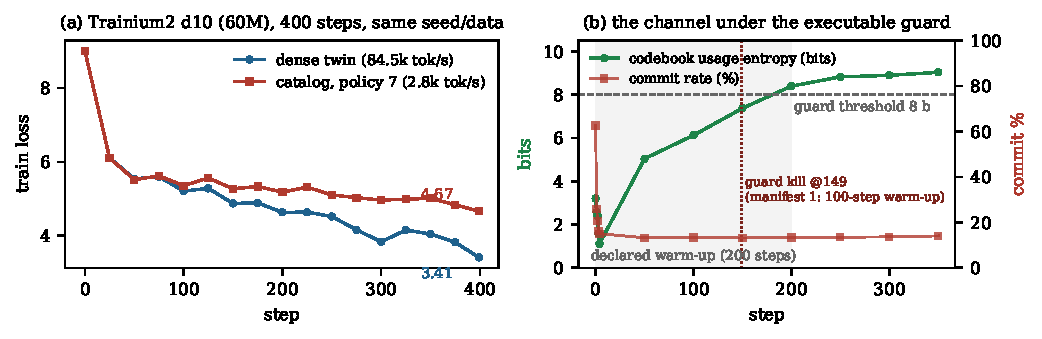
\includegraphics[width=\textwidth]{figs/fig8_trainium.pdf}
  \caption{Third silicon. (a) Trainium2 d10, catalog under policy 7 vs.\ the
  dense twin, same seed and data: 4.67 vs.\ 3.41 at step 399, 2.8k vs.\
  84.5k tok/s. (b) The channel under the executable guard: commit rate
  settles at 13--14\% (one commit per token per unit), codebook usage
  entropy climbs from 1.1 to 9.0 bits; the first manifest's 100-step warm-up
  killed the run at step 149 (entropy 7.36 b, rising), the second, declared
  before the run, allowed 200. \texttt{results/trn2-d10/RESULT.md}.}
  \label{fig:trainium}
\end{figure*}

Getting a lazy compiler to run the write unit at all took six work-arounds,
none of which weakened the contract: every device op in the unit must be
fixed-shape (a dense \texttt{where} mask, not a gather of the
$n_{\text{commits}}$ touched leaves, or the compiler re-traces a NEFF per
step); the STE backward runs on the host from the commit facts (the Neuron
PJRT backward segfaults on it); \texttt{neuronx-cc} 2.26 cannot lower a
top-$k$ over a 32768-wide row for $k\ge16$ (internal assertion; rows
$\le16384$ or $k\le8$ compile, \texttt{sort} is unsupported), so the
proposer takes its top-$M$ in two stages --- within each slot, then over
the $S{\cdot}M$ survivors --- with an explicit composite-key tie-break
(feature-ascending, like the reference; a CPU gate asserts set equality
with the single top-$k$ and zero miss-rate under exact ties); no tensor
shaped $[\cdot, d_{\text{slot}}]$ may exist in the fwd+bwd graph (each is
lowered to one transpose per row: 6M instructions against a 300k limit),
so the apply mask is expanded to leaves on the host, the in-graph clip uses
one-hot matmuls, and the codebook gradient is accumulated on the host,
all-reduced over gloo and uploaded once; and the codebook stays out of the
flat all-reduce bucket. Each is a compiler limit, documented with the
compile-only bisection that found it, not a change to what is verified.

The claim structure widens honestly: NVIDIA+AMD execute \emph{bit-identical
selection} (policies $\le$6, measured); \emph{any} silicon --- including
accelerators we cannot write kernels for --- executes \emph{bit-exactly
verifiable facts} under policy 7.

\begin{figure}[htbp]
  \centering
  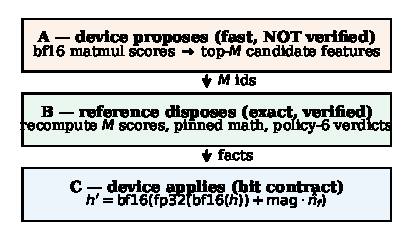
\includegraphics[width=0.95\columnwidth]{figs/fig6_twophase.pdf}
  \caption{Policy 7: device proposes, policy disposes. The verification
  boundary moves; it does not weaken.}
  \label{fig:twophase}
\end{figure}

\section{Journaled inference (instrument only)}
\label{sec:runtime}

The same seam runs at generation time: each emitted token carries the
records of the writes behind it, a confidence signature computed from those
records against training priors, and --- above a calibrated threshold --- a
\textsc{low\_confidence} record committed \emph{before} the token is emitted.
A dead ledger degrades visibly (tokens marked uncitable), never silently.
This is an instrument and a hypothesis, not a result: the planned evaluation
(\S\ref{sec:future}) asks whether confabulation is the inference-time
signature of the structural bypass of \S\ref{sec:collapse}. Nothing in this
paper measures confabulation.

\section{Related work}
\label{sec:related}

\paragraph{Discrete bottlenecks inside transformers.} The closest ancestor
of the catalog is Codebook Features \cite{tamkin2024codebook}: vector-quantized
bottlenecks inserted in every layer of a transformer (up to 410M
parameters), giving sparse, discrete, steerable hidden states at a modest
capacity cost. Backpack LMs \cite{hewitt2023backpack} likewise change the
architecture so that the interior has nameable units. Both train (or
fine-tune) the bottleneck as an \emph{interpretable} object; \sys{} trains it
as a \emph{transactional} one --- writes carry verdicts, the non-write
(\textsc{overflow}/\textsc{abort}) is a first-class fact, and no verdict is
trusted without a bit-exact reference. The channel itself is a VQ-VAE
\cite{oord2017vqvae} trained through a straight-through estimator
\cite{bengio2013ste}, and inherits its known pathology: codebook collapse,
which the VQ literature counters with resets, normalization and better
estimators \cite{huh2023ste}, and the mixture-of-experts literature with
load-balancing losses \cite{shazeer2017moe,fedus2022switch}. Our C4 finding
(\S\ref{sec:collapse}) is the same failure with a twist those settings do not
have: a bypass path let the loss keep falling while the channel was dead, so
the collapse was \emph{silent}. Our answer is not a better estimator but an
executable preregistered guard on commit rate and usage entropy.

\paragraph{Verifiable training.} Proof-of-Learning \cite{jia2021pol} logs
checkpoints and data indices so that a verifier can re-execute segments and
land ``close'' to the next checkpoint; the tolerance band that absorbs GPU
non-determinism is exactly what later spoofing attacks exploited
\cite{zhang2022polattack,fang2023polbroken}. Zero-knowledge proofs of
training \cite{abbaszadeh2024zkpot} remove the tolerance cryptographically
but at minutes of prover time per iteration on a 10M-parameter network. \sys{}
sits at a third design point: no tolerance band (the reference binary makes
every verdict and residual bit-exact across vendors), no cryptographic
succinctness, and a granularity neither has --- the individual 16-byte write
to the residual stream, with \texttt{optimizer.step()} fail-stopped on its
receipt. The receipts are tamper-evident (hash chain), not unforgeable;
combining them with a PoL- or zk-style outer proof is open.

\paragraph{Reading the residual stream after the fact.} The mechanistic
interpretability line --- the residual-stream framing itself
\cite{elhage2021framework}, sparse autoencoders
\cite{bricken2023monosemanticity,cunningham2024sae,templeton2024scaling},
transcoders and attribution graphs \cite{ameisen2025circuit}, and activation
steering \cite{turner2023actadd,zou2023repe} --- estimates what a trained
network writes by fitting a second model to its activations, then tests the
estimate by intervention. Hooking frameworks such as TransformerLens
\cite{nanda2022transformerlens} and the profilers and flight recorders of
distributed training \cite{kineto2020} \emph{observe} the residual stream and
the execution; none makes a write an admitted transaction or a step illegal
without its record. That is the differential: \sys{} does not observe the
residual, it \emph{admits} writes to it, and the record is the
precondition of the step. The two lines are complementary, and we have one
small data point on their overlap: on a wikitext-103 run the journal alone
(no activations read) yields token$\to$feature associations with lifts of
90--178 and purities up to 99.8\% at 5k steps, and denying one such feature
as a journalized \textsc{abort}(policy) raises the NLL of exactly the token it
names ($+0.0032$) and nothing else ($-0.0003$; specificity $10.7\times$;
\texttt{results/probe/}). The effect is small and the model young; the
point is that both the reading and the intervention are records, not
estimates. An SAE trained on the twin could ask what the catalog
\emph{refused} to write.

\paragraph{Open training and documentation requirements.} Fully open
training efforts \cite{groeneveld2024olmo} publish checkpoints, data and
logs --- transparency of artifacts, not machine-checkable evidence of the
process. The EU AI Act \cite{euaiact2024} introduces documentation
obligations for general-purpose AI providers; machine-checkable training
evidence of the kind built here could complement, rather than replace, such
documentation. We make no claim about compliance. The preregistration discipline we borrowed
\cite{nosek2018prereg} is standard in the empirical sciences and, to our
knowledge, not previously applied to a systems paper's own headline.

\section{Limitations and future work}
\label{sec:future}

We name what a capacity claim needs and this paper lacks, so that none of it
is inferred.
\begin{itemize}\itemsep1pt
  \item \textbf{The corrected rerun.} Table~\ref{tab:price} is a run with a
  mis-scaled STE gradient (\S\ref{sec:price}). A d20 rerun with the in-graph
  clip, same manifest, is the experiment that would either keep CORE near
  0.02 --- making the capacity conclusion clean --- or change it.
  \item \textbf{One policy point.} No sweep over $k$, slot width or
  $N_f$; no catalog-as-side-channel arm; no dense bottleneck of matched
  degrees of freedom. ``The configuration tested is too narrow'' is the
  supported statement; ``the architecture is'' is not.
  \item \textbf{Generality of the collapse.} Shown on one host architecture
  whose declared bypass scalars can carry the loss (\S\ref{sec:collapse}).
  \item \textbf{Throughput.} $12$--$29\times$ the twin. The two-phase cost
  is the per-unit host round trip; a two-pass forward (propose every unit,
  dispose once, apply once) is the lever and is not built.
  \item \textbf{Retention.} Raw records are sampled (1/100 steps); chains
  and counts are durable. Selective retention policies are future work.
  \item \textbf{Integrity, not non-repudiation.} Receipts are tamper-evident
  hash-chain heads, forgeable by whoever runs the seam; keying or external
  anchoring is not built.
  \item \textbf{Planned evaluation: confabulation as bypass.} Signatures
  F1--F9 over write records, a knowledge-boundary task with mechanical labels
  drawn from the model's own training shards, a preregistered AUROC $\ge
  0.65$ gate, and the hypothesis that confabulation is the inference-time
  form of \S\ref{sec:collapse}. Designed and instrumented; not run, and it
  requires a cataloged model that knows something --- the d20 model of
  \S\ref{sec:price} does not. Reported when it exists, in either direction.
  \item \textbf{The SFT that exposed the bug.} After the fix, SFT of the d20
  catalog ran cleanly (466 steps, val bpb 0.875, channel alive); its chat
  evaluation is at chance (ARC-E 25.6\%, ARC-C 24.4\%, MMLU 25.5\%),
  consistent with \S\ref{sec:price}. The Trainium2 d10 run
  (\S\ref{sec:twophase}) is a corrected-mirror run at a smaller scale; no
  CORE evaluation of its checkpoints has been done.
\end{itemize}

\section*{Acknowledgements}
This work trained inside nanochat \cite{karpathy2025nanochat}, Andrej Karpathy's
from-scratch LLM pipeline; every d12/d20 number here was obtained with nanochat
as the host trainer, the dense twin is unmodified nanochat, and CORE is
nanochat's \texttt{base\_eval}. We integrate by an additive patch against a
pinned commit and redistribute none of it. The Trainium2 experiments ran on the
AWS Neuron team's nanochat competition tree and toolchain; the AMD runs on
DigitalOcean MI355X spot capacity.

\section{Evidence table}
\label{sec:evidence}

\begin{table}[h]
\scriptsize
\centering
\begin{tabular}{@{}ll@{}}
\toprule
Claim & Evidence path \\
\midrule
Cross-vendor gate & \texttt{results/gates/\{NVIDIA-H100,AMD-MI355X\}} \\
36/36 injection & \texttt{results/inject/inject-summary.json} \\
1b PASS + seeds & \texttt{results/train/NVIDIA-H200/seeds-*} \\
LR-sweep reversal & \texttt{results/train/NVIDIA-H200/lrsweep-*} \\
AMD replication & \texttt{results/train/AMD-*-phase1b-*} \\
d12 DDP 8-rank & \texttt{results/nanochat/AMD-8xMI355X-d12-3.3} \\
Channel collapse & \texttt{results/nanochat/PHASE5-CHANNEL-*.md} \\
Kill-test resume & \texttt{results/nanochat/KILLTEST-PASS.md} \\
Phase-5 price (CORE) & \texttt{results/models/d20-p5/RESULT.md}, S3 \\
Two-phase gate & \texttt{python/tests/test\_two\_phase.py} \\
Trainium2 d10 catalog vs twin & \texttt{results/trn2-d10/}, S3 \\
Neuron compiler findings & \texttt{results/gates/AWS-Trainium2/} \\
Semantic probe & \texttt{results/probe/semantics-v0.json} \\
\bottomrule
\end{tabular}
\caption{Every quantitative claim maps to a committed artifact; ledger keys
cited inside each NOTES file.}
\end{table}

\begin{thebibliography}{99}\footnotesize
\bibitem{tamkin2024codebook} A.~Tamkin, M.~Taufeeque, N.~D. Goodman. Codebook Features: Sparse and Discrete Interpretability for Neural Networks. \emph{ICML}, 2024.
\bibitem{hewitt2023backpack} J.~Hewitt, J.~Thickstun, C.~D. Manning, P.~Liang. Backpack Language Models. \emph{ACL}, 2023.
\bibitem{oord2017vqvae} A.~van den Oord, O.~Vinyals, K.~Kavukcuoglu. Neural Discrete Representation Learning. \emph{NeurIPS}, 2017.
\bibitem{bengio2013ste} Y.~Bengio, N.~L\'eonard, A.~Courville. Estimating or Propagating Gradients Through Stochastic Neurons for Conditional Computation. arXiv:1308.3432, 2013.
\bibitem{huh2023ste} M.~Huh, B.~Cheung, P.~Agrawal, P.~Isola. Straightening Out the Straight-Through Estimator: Overcoming Optimization Challenges in Vector Quantized Networks. \emph{ICML}, 2023.
\bibitem{shazeer2017moe} N.~Shazeer et al. Outrageously Large Neural Networks: The Sparsely-Gated Mixture-of-Experts Layer. \emph{ICLR}, 2017.
\bibitem{fedus2022switch} W.~Fedus, B.~Zoph, N.~Shazeer. Switch Transformers: Scaling to Trillion Parameter Models with Simple and Efficient Sparsity. \emph{JMLR}, 23(120), 2022.
\bibitem{jia2021pol} H.~Jia et al. Proof-of-Learning: Definitions and Practice. \emph{IEEE S\&P}, 2021.
\bibitem{zhang2022polattack} R.~Zhang et al. ``Adversarial Examples'' for Proof-of-Learning. \emph{IEEE S\&P}, 2022.
\bibitem{fang2023polbroken} C.~Fang et al. Proof-of-Learning is Currently More Broken Than You Think. \emph{IEEE EuroS\&P}, 2023.
\bibitem{abbaszadeh2024zkpot} K.~Abbaszadeh, C.~Pappas, J.~Katz, D.~Papadopoulos. Zero-Knowledge Proofs of Training for Deep Neural Networks. \emph{ACM CCS}, 2024.
\bibitem{elhage2021framework} N.~Elhage et al. A Mathematical Framework for Transformer Circuits. \emph{Transformer Circuits Thread}, 2021.
\bibitem{bricken2023monosemanticity} T.~Bricken et al. Towards Monosemanticity: Decomposing Language Models With Dictionary Learning. \emph{Transformer Circuits Thread}, 2023.
\bibitem{cunningham2024sae} H.~Cunningham, A.~Ewart, L.~Riggs, R.~Huben, L.~Sharkey. Sparse Autoencoders Find Highly Interpretable Features in Language Models. \emph{ICLR}, 2024.
\bibitem{templeton2024scaling} A.~Templeton et al. Scaling Monosemanticity: Extracting Interpretable Features from Claude 3 Sonnet. \emph{Transformer Circuits Thread}, 2024.
\bibitem{ameisen2025circuit} E.~Ameisen et al. Circuit Tracing: Revealing Computational Graphs in Language Models. \emph{Transformer Circuits Thread}, 2025.
\bibitem{turner2023actadd} A.~M. Turner et al. Activation Addition: Steering Language Models Without Optimization. arXiv:2308.10248, 2023.
\bibitem{zou2023repe} A.~Zou et al. Representation Engineering: A Top-Down Approach to AI Transparency. arXiv:2310.01405, 2023.
\bibitem{karpathy2025nanochat} A.~Karpathy. nanochat: the best ChatGPT that \$100 can buy --- a full-stack LLM training and inference pipeline. \url{https://github.com/karpathy/nanochat}, 2025.
\bibitem{nanda2022transformerlens} N.~Nanda, J.~Bloom. TransformerLens: A Library for Mechanistic Interpretability of Generative Language Models. \url{https://github.com/TransformerLensOrg/TransformerLens}, 2022.
\bibitem{kineto2020} PyTorch Kineto: CPU+GPU profiling library, and the PyTorch Flight Recorder for collective operations. \url{https://github.com/pytorch/kineto}, 2020--2025.
\bibitem{groeneveld2024olmo} D.~Groeneveld et al. OLMo: Accelerating the Science of Language Models. \emph{ACL}, 2024.
\bibitem{euaiact2024} European Parliament and Council. Regulation (EU) 2024/1689 (Artificial Intelligence Act), Art.~53 and Annex~XI, 2024.
\bibitem{nosek2018prereg} B.~A. Nosek, C.~R. Ebersole, A.~C. DeHaven, D.~T. Mellor. The Preregistration Revolution. \emph{PNAS}, 115(11), 2018.
\end{thebibliography}

\end{document}
